\documentclass[12pt,letterpaper]{article}
\usepackage{fullpage}
\usepackage[top=2cm, bottom=4.5cm, left=2.5cm, right=2.5cm]{geometry}
\usepackage{amsmath,amsthm,amsfonts,amssymb,amscd}
\usepackage{lastpage}
\usepackage{enumerate}
\usepackage{fancyhdr}
\usepackage{mathrsfs}
\usepackage{xcolor}
\usepackage{graphicx}
\usepackage{listings}
\usepackage{hyperref}
\usepackage{soul}
\usepackage{pgfplots}

\hypersetup{%
  colorlinks=true,
  linkcolor=blue,
  linkbordercolor={0 0 1}
}
 
\renewcommand\lstlistingname{Algorithm}
\renewcommand\lstlistlistingname{Algorithms}
\def\lstlistingautorefname{Alg.}

\newcommand{\sur}[1]{\ensuremath{^{\textrm{#1}}}}
\newcommand{\sous}[1]{\ensuremath{_{\textrm{#1}}}}

\lstdefinestyle{Python}{
    language        = Python,
    frame           = lines, 
    basicstyle      = \footnotesize,
    keywordstyle    = \color{blue},
    stringstyle     = \color{green},
    commentstyle    = \color{red}\ttfamily
}

\setlength{\parindent}{0.0in}
\setlength{\parskip}{0.05in}

% Edit these as appropriate
\newcommand\course{CSCI 2400}      %<--class
\newcommand\hwnumber{7}                  % <-- homework number
\newcommand\NetIDa{Rhett Hanscom}           % <-- NetID of person #1
\newcommand\NetIDb{rhha1623@colorado.edu}           % <-- NetID of person #2 (Comment this line out for problem sets)

\pagestyle{fancyplain}
\headheight 35pt
\lhead{\NetIDa}
\lhead{\NetIDa\\\NetIDb}                 % <-- Comment this line out for problem sets (make sure you are person #1)
\chead{\textbf{\Large Homework \hwnumber}}
\rhead{\course \\ \today}
\lfoot{}
\cfoot{}
\rfoot{\small\thepage}
\headsep 1.5em

\begin{document}

\section*{Problem 12.18}

\begin{figure}[!h]
    \centering
    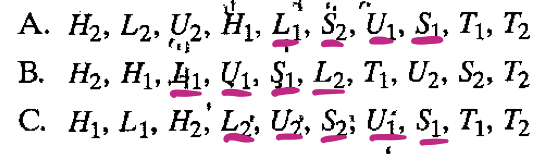
\includegraphics[width=1\linewidth]{1218.jpg}
    \caption{Table from question 12.18 in the text, with the steps in the sequence which make these paths unsafe underlined..}
    \end{figure}
 
\section*{Problem 12.29}

As each of the sets between Thread 1 and Thread 2 are disjointed, there is no risk of deadlock occuring in this scenario.

\newpage
\section*{Problem 12.16}

\begin{verbatim}
#include "csapp.h"
void *thread(void *vargp);

int main(int argc, char *argv[]){
    pthread_t tid;
    long argnumber = strtol(argv[1], NULL, 0);

    for (int i = 0; i < argnumber; i++){
        pthread_create(&tid, NULL, thread, NULL);
        pthread_join(tid, NULL);
    }
    exit(0);
}

void *thread(void *vargp){
    printf("Hello, world!\n");
    return NULL;
}
\end{verbatim}

\end{document}
